\chapter{Theoretical Analysis} \label{chap:theoretical-analysis}

In this chapter, we start from the fluid description of plasma, and derive the governing equations for the flow in magnetic nozzle. After this, we linearize the governing equations and reformulate the problem as a polynomial eigenvalue problem. Then a special case is discussed analytically.

\section{Fluid Description for Flow}
In this section, we will derive the governing equations of the flow in magnetic nozzle, starting from the fluid description for plasma.

We start by deriving the usefule form of the conservation of density,
\[ \pdv{n}{t} + \div(n\mathbf{v}) = 0 \]
where $\mathbf{v}$ here denotes the fluid velocity of the plasma flow.

We can get the fluid velocity by taking the integral
\[ \mathbf{v} = \frac{1}{n}\int_{\mathbb{R}^3} \mathbf{v}_p f(\mathbf{x}, \mathbf{v}_p, t) d^3\mathbf{v}_p \]

Denote the particle velcity as $\mathbf{v}_p$, we can decompose the particle velocity vector as $\mathbf{v}_p = (v_\parallel,v_\perp)$, where $v_\parallel$ and $v_\perp$ are the magnitudes of components that are parallel to and perpendicular to the magnetic field line, respectively. Due to the Lorentz force, the charged particles gyrates about the magnetic field lines, see Fig.~\ref{fig:gyrate-along-b-field}. Hence, the $v_\perp$ will be averaged to zero the expression for plasma fluid velocity can be simplied as
\[\mathbf{v} = v\mathbf{B}/B\]
where $v$ is the fluid speed along the magnetic field lines. This makes sence because the charged particles flows along $\mathbf{B}$.

By expanding the divergence term, and using the divergence free condition $\div B=0$, we have
\[ \pdv{n}{t} + \mathbf{B}\cdot \grad(\frac{nv}{B}) = 0 \]
Since the magnetic field lines are aligned with the central axis of the nozzle, which we denote as z-axis, so $\mathbf{B} = B\hat{z}$. Now we obtain the conservation of density for the magnetic nozzle,
\begin{equation}
	\pdv{n}{t} + B\pdv{z}(\frac{nv}{B}) = 0
\end{equation}

The second governing equation is the conservation of momentum,
\[ mn\pdv{\mathbf{v}}{t} + mn\mathbf{v}\cdot\grad\mathbf{v} = -\grad p \]
where $m$ is the ion mass. This equation tells us the plasma flow is driven by pressure.

The equation of state is given by the isothermal condition,
\begin{equation} \label{eq:eos}
	p = nk_BT
\end{equation}
There are two main reasons. First the plasma particles are confined to the magnetic field lines. This reduces the particle collisions and energy exchanges. Moreover, the electrons have high mobility, they will quickly fill up any charge cavities and thus maintain a constant temperature. Hence, we can safely assume the plasma flow is isothermal.

Therefore, we have
\begin{equation}
	\pdv{v}{t} + v\pdv{v}{z} = -c_s^2\frac{1}{n}\pdv{n}{z}
\end{equation}
where $c_s^2 = k_BT/m$ is the square of sound speed.

Therefore, the dynamics of the plasma flow in magnetic nozzle can be characterized by the conservation of density and momentum,
\begin{align*}
	 & \pdv{n}{t} + B\pdv{z}(\frac{nv}{B}) = 0                \\
	 & \pdv{v}{t} + v\pdv{v}{z} = -c_s^2\frac{1}{n}\pdv{n}{z}
\end{align*}
The magnetic field profile was discussed in Sec.\ref{sec:magnetic-field-in-nozzle}.

In this research, we are interested in the stability of the equilibrium flow in the nozzle. Let's denote $n_0$ and $v_0$ as equilibrium density and equilibrium velocity, respectively. Since they are stationary (time independent) solutions to the above set of equations, so they satisfy the so-called equilibrium condition,
\begin{align*}
	 & B\pdv{z}(\frac{n_0v_0}{B})  = 0                   \\
	 & v_0\pdv{v_0}{z} = -c_s^2\frac{1}{n_0}\pdv{n_0}{z}
\end{align*}

\section{Non-dimensionalization}
For convenience, we nondimensionalize the governing equations by normalizing the velocity to $c_s$, $v\mapsto v/c_s$, $z$ to system length $L$, $z \mapsto z/L$ and time $t\mapsto c_s t/L$. The governing equations become
\begin{align}
	 & \pdv{n}{t} + n\pdv{v}{z} + v\pdv{n}{z} - nv\frac{\partial_z B}{B} = 0
	\label{eq:conservation-of-density}
	\\
	 & n\pdv{v}{t} + nv\pdv{v}{z} = -\pdv{n}{z}
	\label{eq:conservation-of-momentum}
\end{align}
and the nondimensionalized equilibrium condition is
\begin{align}
	 & \pdv{z}(\frac{n_0v_0}{B}) = 0 \label{eq:equilibrium-conservation-of-density}                 \\
	 & v_0\pdv{v_0}{z} = -\frac{1}{n_0}\pdv{n_0}{z} \label{eq:equilibrium-conservation-of-momentum}
\end{align}

\section{Velocity Profiles at Equilibrium}
In this section we will solve the equilibrium velocity profile, $v_0$, from the nondimensionalized equilibrium condition, Eq.~(\ref{eq:equilibrium-conservation-of-density}) and Eq.~(\ref{eq:equilibrium-conservation-of-momentum}).
We start by substituting $\frac{1}{n_0}\pdv*{n_0}{z}$ into Eq.~(\ref{eq:equilibrium-conservation-of-density}), then it becomes
\[ (v_0^2-1)\pdv{v_0}{z} = -\frac{v_0}{B}\pdv{B}{z} \]

Notice that there is a singularity at $v_0=1$, the sonic speed.

This is a separable equation, integrate it and use the conditions at midpoint $B(0)=B_m, v_0(0)=v_m$ we get
\[ v_0^2e^{-v_0^2} = \frac{B^2}{B_m^2}v_m^2e^{-v_m^2} \]
We can now express $v_0$ using the Lambert W function (see Appendix \ref{app:lambert-w}),
\begin{equation}
	v_0(z) = \left[ -W_k\left(-\frac{B(z)^2}{B_m^2}v_m^2e^{-v_m^2}\right) \right]^{1/2}
	\label{eq:velocity-profile}
\end{equation}
where the subscript $k$ of $W$ stands for branch of Lambert W function.

When considering the velocity profile of a nozzle flow, various scenarios can be distinguished based on the Mach number parameter ($v_m$) and the branch ($k$) used in the expression for the Mach number distribution, denoted as $v_0(z)$. These parameters play a crucial role in determining the flow characteristics. The selection of appropriate $v_m$ and $k$ values facilitates the control of the flow characteristics in the nozzle, allowing for the realization of various flow regimes, such as subsonic, supersonic, transonic, accelerating, or decelerating profiles. Different velocity profiles are shown in Fig.~\ref{fig:velocity-profiles}.

Firstly, for the case where $v_m < 1$ and $k = 0$, the resulting velocity profile is classified as subsonic. This means that both at the entrance and exit of the nozzle, the velocity remains subsonic, and the midpoint velocity is also less than unity ($v_m < 1$). A subsonic flow is characterized by fluid velocities that are slower than the local speed of sound.

On the other hand, when $v_m > 1$ and $k = -1$, the velocity profile corresponds to a supersonic flow regime. In this situation, the fluid velocities at both the entrance and exit of the nozzle are supersonic, and the midpoint velocity ($v_m$) exceeds the value of unity ($v_m > 1$). Supersonic flow is characterized by velocities that surpass the speed of sound.

Furthermore, when $v_m = 1$, the velocity profile becomes transonic. In this case, the midpoint velocity is exactly at the sonic threshold ($v_m = 1$), where the fluid velocity equals the local speed of sound. Transonic flows often exhibit a combination of subsonic and supersonic regions, and this regime poses unique challenges due to the presence of singularity at the nozzle throat. We will discuss this thoroughly in Chap.~\ref{chap:singular-perturbation}.

To achieve an accelerating velocity profile, a configuration with $k = 0$ for $x < 0$ and $k = -1$ for $x > 0$ is employed. Here, $x$ represents the spatial coordinate along the nozzle length. With this setup, the flow starts subsonically and gradually accelerates to a supersonic speed as it propagates along the nozzle.

Conversely, a decelerating velocity profile can be obtained by adopting a similar approach but with reversed values of $k$. Specifically, the configuration will have $k = -1$ for $x < 0$ and $k = 0$ for $x > 0$, causing the flow to start supersonically and decelerate to subsonic velocities further down the nozzle.

\begin{figure}[H]
	\centering
	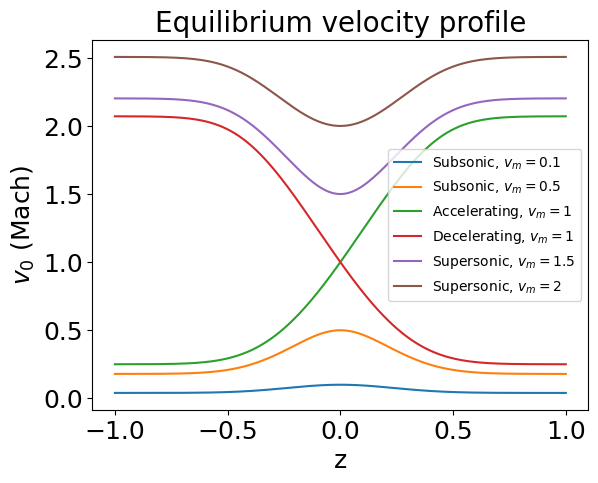
\includegraphics[width=0.7\linewidth]{figures/velocity-profiles}
	\caption{The velocity profile in the magnetic nozzle is completely determined by the midpoint mach number $v_m$ and the branch $k$. A subsonic profile can be obtained by selecting $v_m<1$ and $k=0$. On the other hand, a supersonic profile can be obtained by setting $v_m>1$ and $k=-1$. Lastly, for the transonic velocity profiles, the midpoint velocity is set to unity, $v_m=1$, and then by choose $k=0$ for $x<0$ and $k=-1$ for $x>0$ we get accelerating profile. Decelerating profile can be obtained similarly.}
	\label{fig:velocity-profiles}
\end{figure}

\section{Linearized Governing Equations}
As illustrated in Sec.\ref{sec:two-stream-instability}, it is essential to linearize the governing equations in order to investigate the instability of plasma. Now we are going to derive the linearized governing equations with the equilibrium conditions given in above.

Let $n = n_0(z) + \tilde{n}(z,t)$ and $v = v_0(z) + \tilde{v}(z,t)$, where $\tilde{n}$ and $\tilde{v}$ are small perturbed quantities.

We first linearize Eq.~(\ref{eq:conservation-of-density}) by setting $n=n_0+\tilde{n}$ and $v=v_0+\tilde{v}$,
\[    \pdv{(n_0+\tilde{n})}{t}
	+ (n_0+\tilde{n})\pdv{(v_0+\tilde{v})}{z}
	+ (v_0+\tilde{v})\pdv{(n_0+\tilde{n})}{z}
	- (n_0+\tilde{n})(v_0+\tilde{v})\frac{\partial_z B}{B} = 0
\]
By ignoring the second order perturbations, we obtain
\[ \frac{1}{n_0}\pdv{\tilde{n}}{t}
	+ \pdv{v_0}{z} + \frac{\tilde{n}}{n_0}\pdv{v_0}{z} + \pdv{\tilde{v}}{z}
	+ \frac{v_0}{n_0}\pdv{n_0}{z} + \frac{\tilde{v}}{n_0}\pdv{n_0}{z} + \frac{v_0}{n_0}\pdv{\tilde{n}}{z}
	- v_0\frac{\partial_z B}{B} - \tilde{v}\frac{\partial_z B}{B} - \tilde{n}\frac{v_0}{n_0}\frac{\partial_z B}{B} = 0
\]


Using the equilibrium condition Eq.~(\ref{eq:equilibrium-conservation-of-density}), some of the terms are canceled. Moreover, the last term can be written as
\[ \tilde{n}\frac{v_0}{n_0}\frac{\partial_z B}{B} = \frac{\tilde{n}}{n_0}\left( \frac{\partial_z n_0}{n_0}v_0 + \pdv{v_0}{z} \right) \]
Now, we get the linearized conservation of mass,
\begin{equation} \label{eq:linearized-conservation-of-density}
	\frac{1}{n_0}\pdv{\tilde{n}}{t}
	+ \pdv{\tilde{v}}{z} + v_0\tilde{Y} + \tilde{v}\frac{\partial_z n_0}{n_0} - \tilde{v}\frac{\partial_z B}{B} = 0
\end{equation}
where
\[ \tilde{Y} \equiv \frac{1}{n_0}\pdv{\tilde{n}}{z} - \frac{\partial_z n_0}{n_0^2}\tilde{n} = \pdv{z}(\frac{\tilde{n}}{n_0}) \]

To linearize the conservation of momentum, we follow the same logic by substituting $n=n_0+\tilde{n}$, and $v=v_0+\tilde{v}$ in Eq.~(\ref{eq:conservation-of-momentum}),
\[ (n_0+\tilde{n})\pdv{(v_0+\tilde{v})}{t} + (n_0+\tilde{n})(v_0+\tilde{v})\pdv{(v_0+\tilde{v})}{z} = -\pdv{n}{z} \]

Again, ignore second order perturbations and rearange terms, we have
\[ \pdv{v_0}{t} + v_0\pdv{v_0}{z} + \tilde{v}\pdv{v_0}{z}
	= -\frac{1}{n_0}\pdv{n_0}{z} -\frac{1}{n_0}\pdv{\tilde{n}}{z} -v_0\frac{v_0}{z} - \frac{\tilde{n}}{n_0}v_0\pdv{v_0}{z} \]
Using the equilibrium condition Eq.~(\ref{eq:equilibrium-conservation-of-momentum}) on the RHS, we get the linearized conservation of momentum,
\begin{equation} \label{eq:linearized-conservation-of-momentum}
	\pdv{\tilde{v}}{t} + \pdv{(v_0\tilde{v})}{z} = -\tilde{Y}
\end{equation}

\section{Polynomial Eigenvalue Problem}
We can further simplify the problem by combining Eq.~(\ref{eq:linearized-conservation-of-density}) and Eq.~(\ref{eq:linearized-conservation-of-momentum}) into a single equation. We can substitute Eq.~(\ref{eq:linearized-conservation-of-momentum}) into Eq.~(\ref{eq:linearized-conservation-of-density}) to eliminate $\tilde{Y}$,

\begin{equation} \label{eq:single-governing-equation}
	\pdv{t}\frac{\tilde{n}}{n_0}
	+ \pdv{\tilde{v}}{z} - v_0\left(\pdv{t}\tilde{v}
	+ \pdv{(v_0\tilde{v})}{z}\right)
	+ \tilde{v}\frac{\partial_z n_0}{n_0}
	- \tilde{v}\frac{\partial_z B}{B}
	= 0
\end{equation}

In order to investigate the instability of the flow, we need formulate it as an eigenvalue problem. To do that, we assume the perturbed density and velocity are oscillatory, i.e. $\tilde{n}, \tilde{v} \sim \exp(-i\omega t)$, where $\omega$ is the oscillation frequency of the perturbed quantities. This frequency can be a complex number.

As illustrated in Sec.\ref{sec:two-stream-instability}, the flow can be stable or unstable depending on the imaginary part of the frequency. If $\Im(\omega) > 0$, then the perturbed quantities $\tilde{n} \sim \exp(\Im(\omega) t)$, which means it grows exponentially with time, hence unstable. If $\Im(\omega) \leq 0$, then the amplitude of the perturbed quanties are either unchanged or exponentially decreasing, hence the flow is stable.

By assuming oscillatory perturbed quantities, Eq.~(\ref{eq:single-governing-equation}) becomes,
\begin{equation}
	-i\omega\frac{\tilde{n}}{n_0}
	+ \pdv{\tilde{v}}{z} - v_0\left(-i\omega\tilde{v}
	+ \pdv{(v_0\tilde{v})}{z}\right)
	+ \tilde{v}\frac{\partial_z n_0}{n_0}
	- \tilde{v}\frac{\partial_z B}{B}
	= 0
\end{equation}

Using the equilibrium condition Eq.~(\ref{eq:equilibrium-conservation-of-density}), we can eliminate the term $\partial_z B/B$,
\[
	-i\omega\frac{\tilde{n}}{n_0}
	+ \pdv{\tilde{v}}{z}
	+ v_0\left(i\omega \tilde{v} - v_0\pdv{\tilde{v}}{z} - \tilde{v}\pdv{v_0}{z} \right)
	- \tilde{v}\frac{\partial_z v_0}{v_0}
	= 0
\]

Rearrange terms, we have
\[
	-i\omega\frac{\tilde{n}}{n_0}
	+ i\omega v_0\tilde{v}
	+ (1-v_0^2)\pdv{\tilde{v}}{z}
	- \left(v_0+\frac{1}{v_0}\right)\pdv{v_0}{z}\tilde{v} = 0
\]

Now we take $\pdv*{t}$ on Eq.~(\ref{eq:linearized-conservation-of-momentum}). Recall the fact that $\tilde{Y} = \partial_z(\tilde{n}/n_0)$, we have
\[
	\omega^2\tilde{v} + i\omega\left(v_0\pdv{\tilde{v}}{z} + \tilde{v}\pdv{v_0}{z}\right)
	= \pdv{t}\pdv{z}(\frac{\tilde{n}}{n_0})
\]
Apply $\partial_t$ operator first, we get
\[
	\omega^2\tilde{v} + i\omega\left(v_0\pdv{\tilde{v}}{z} + \tilde{v}\pdv{v_0}{fz}\right)
	= \pdv{z}(-i\omega v_0\tilde{v}
	- (1-v_0^2)\pdv{\tilde{v}}{z}
	+ \left(v_0+\frac{1}{v_0}\right)\pdv{v_0}{z}\tilde{v})
\]
Expand the RHS and collect terms, we get
\begin{equation} \label{eq:polynomial-eigenvalue-problem}
	\begin{aligned}
		 & \omega^2 \tilde{v}                                          \\
		 & +2i\omega\left(v_0\pdv{}{z} + \pdv{v_0}{z}\right) \tilde{v} \\
		 & +\left[ (1-v_0^2)\pdv[2]{}{z}
			-\left(3v_0 + \frac{1}{v_0}\right)\pdv{v_0}{z}\pdv{}{z}
			- \left(1-\frac{1}{v_0^2}\right)\left(\pdv{v_0}{z}\right)^2
			- \left(v_0+\frac{1}{v_0}\right)\pdv[2]{v_0}{z} \right]\tilde{v}
		= 0
	\end{aligned}
\end{equation}

In mathematical terms, Eq.~(\ref{eq:polynomial-eigenvalue-problem}) is a polynomial eigenvalue problem, where $\omega$ is an eigenvalue to the problem, and the velocity perturbation $\tilde{v}$ is an eigenfunction associated with the eigenvalue $\omega$. In the later chapters we will discuss the methods to tackle this problem.

\section{Analytical Solutions to Constant Velocity Case}
In this section we are going to tackle the simplest case of the polynomial eigenvalue problem, Eq.~(\ref{eq:polynomial-eigenvalue-problem}), the constant velocity case.

The constant velocity profile can be viewed as the limit of $v_0(z)$ as the spread of magnetic field goes to infinity, $\delta\to\infty$. As the parameter $\delta$ approaches infinity, the width of the magnetic field enlarges and eventually becomes flat. In other words, a constant magnetic field. We can easily see that the velocity profile $v_0(z)$ becomes a constant as well.

If we set the velocity profile of the equilibrium flow to constant $v_0=\text{const}$, then Eq.~(\ref{eq:polynomial-eigenvalue-problem}) becomes a simple boundary value problem with second order constant coefficients differential equation.

\begin{equation} \label{eq:constant-v-problem-dirichlet}
	\omega^2\tilde{v} + 2i\omega v_0\pdv{\tilde{v}}{z} + (1-v_0^2)\pdv[2]{\tilde{v}}{z} = 0
\end{equation}

We need two boundary values in order to uniquely determine the solution (up to a constant). In the following subsections, we will solve Eq.~(\ref{eq:polynomial-eigenvalue-problem}) with constant velocity under two sets of boundary conditions, Dirichlet and fixed-open boundary condition.

\subsection{Dirichlet Boundary}
In this subsection, the so-called Dirichlet boundary condition will be used. It has the name because the function values are fixed at the two ends of the nozzle,
\[ \tilde{v}(-1) = \tilde{v}(1) = 0 \]
At the left end (entrance of the nozzle), $z=-1$, we assume there are no perturbations. As for the right end (exit of the nozzle), $z=1$, setting the velocity perturbation to 0 might not be the best boundary condition to describe the physical process of the plasma flow in the nozzle, it nevertheless serves as a starting point to the problem.

With the two boundary conditions, we are able to determine the solution to this problem,
\begin{equation} \label{eq:constant-v-solution-dirichlet}
	\tilde{v}(z) = C\left[ \exp\left(i\omega\frac{z+1}{v_0+1}\right) - \exp\left(i\omega\frac{z+1}{v_0-1}\right) \right]
\end{equation}
where $C\in\mathbb{C}$ is a complex constant, and the frequencies are $\omega=n\pi(1-v_0^2)/2$ with $n\in\mathbb{Z}$. The results are plotted in Fig.~\ref{fig:exact-v-dirichlet} This result tells us that the flow in magnetic nozzle is stable regardless the velocity $v_0$ for constant velocity case. It is worth to mention $v_0=1$ is a singular point of this problem.

This solution is exact, we will use this to benchmark the simulation results in later chapter.

\begin{figure}[htbp]
	\centering
	\begin{subfigure}{0.5\textwidth}
		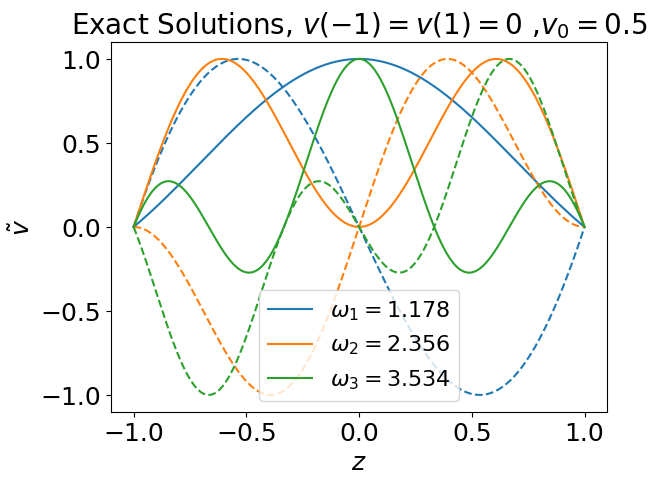
\includegraphics[width=\linewidth]{figures/exact-fixed-fixed-v0=0.5}
		\caption{Subsonic}
	\end{subfigure}%
	\begin{subfigure}{0.5\textwidth}
		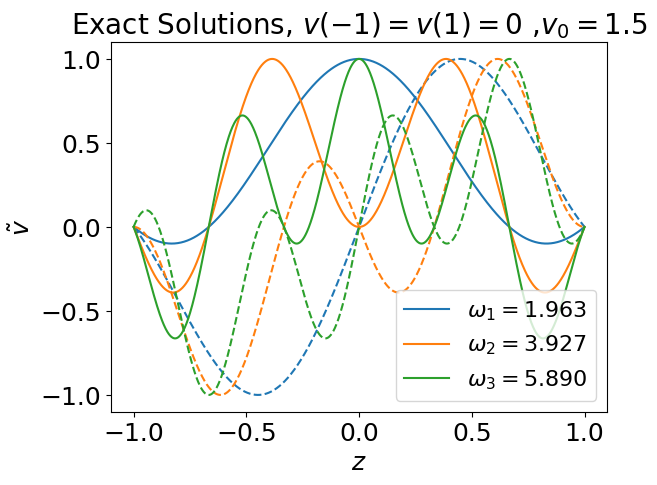
\includegraphics[width=\linewidth]{figures/exact-fixed-fixed-v0=1.5}
		\caption{Supersonic}
	\end{subfigure}
	\caption{The plots show the first three non-zero exact solutions to Eq.~(\ref{eq:constant-v-problem-dirichlet}) for both subsonic and supersonic case. These solutions are stable.}
	\label{fig:exact-v-dirichlet}
\end{figure}

\subsection{Fixed-Open Boundary}
Fixed-Open boundary condition assumes that there are no perturbations at the entrance of the nozzle, and it is free on the exit of the nozzle.

\begin{equation} \label{eq:constant-v-problem-fixed-open}
	\omega^2\tilde{v} + 2i\omega v_0\pdv{\tilde{v}}{z} + (1-v_0^2)\pdv[2]{\tilde{v}}{z} = 0
	\quad
	\tilde{v}(-1) = \pdv{\tilde{v}}{z}\,(1) = 0
\end{equation}

The solution to this problem is
\begin{equation} \label{eq:constant-v-solution-fixed-open}
	\tilde{v}(z) = C\left(\exp\left(i\omega\frac{z+1}{v_0+1}\right)
	- \exp\left(i\omega\frac{z+1}{v_0-1}\right)\right)
\end{equation}
where $C\in\mathbb{C}$ is a complex constant, and $\omega = (v_0^2 - 1) \left[\frac{n\pi}{2} - \frac{1}{4}i\ln(\frac{v_0-1}{v_0+1})\right]$ with $n\in\mathbb{Z}$. The term $i\ln((v_0-1)/(v_0+1))\in\mathbb{C}$ and its imaginary part is positive for any $v_0\neq 1$. Therefore,
\begin{itemize}
	\item If $v_0<1$, then $\Im(\omega)<0$, it's damped oscillation, hence stable.
	\item If $v_0>1$, then $\Im(\omega)>0$, it's unstable.
\end{itemize}

Worth to mention, this is a very interesting solution with the following properties,
\begin{enumerate}
	\item The growth rate is independent the mode number $n$.
	\item The ground mode $n=0$ for subsonic case has non-zero real part and imaginary part.
\end{enumerate}

\begin{figure}[htbp]
	\centering
	\begin{subfigure}{0.5\textwidth}
		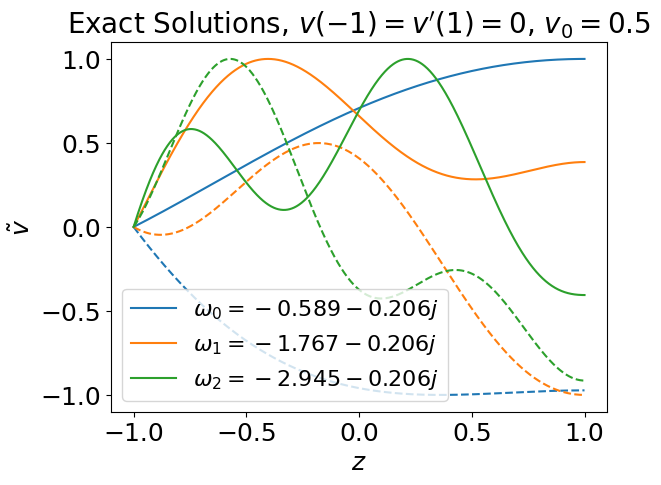
\includegraphics[width=\linewidth]{figures/exact-fixed-open-v0=0.5}
		\caption{Subsonic, stable flow.}
	\end{subfigure}%
	\begin{subfigure}{0.5\textwidth}
		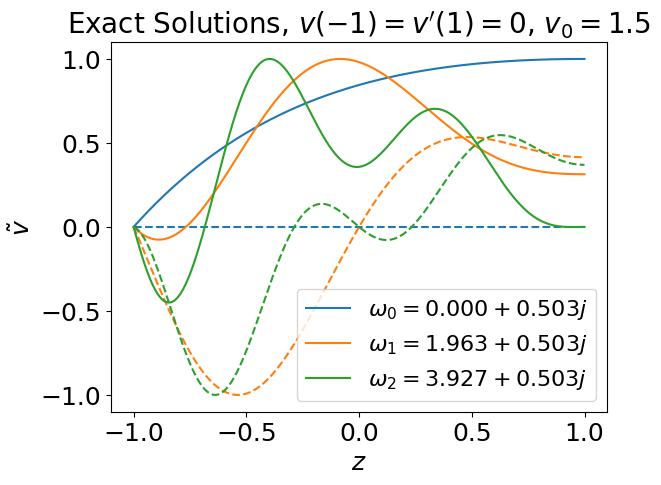
\includegraphics[width=\linewidth]{figures/exact-fixed-open-v0=1.5}
		\caption{Supersonic, unstable flow.}
	\end{subfigure}
	\caption{The plots show the first three exact solutions to Eq.~(\ref{eq:constant-v-problem-fixed-open}) for both subsonic and supersonic case. The flow is stable for subsonic case and unstable for supersonic case.}
	\label{fig:exact-v-fixed-open}
\end{figure}
